\documentclass[a4,12pt]{article}
\usepackage[margin=0.5in]{geometry}
\usepackage{titlesec}
\usepackage{ifthen}
\usepackage{fancyhdr}
\usepackage{amsmath}
\usepackage{amssymb}
\usepackage{systeme}
\usepackage{amsfonts}
\usepackage[utf8]{inputenc}
\usepackage[T1]{fontenc}
\usepackage[polish,english]{babel}
\usepackage{graphicx}
\usepackage{subfig}
\usepackage{caption}

% -------- %
% SECTIONS %
% -------- %
\newcounter{problemnumber}\setcounter{problemnumber}{1}
\titlespacing\section{5pt}{15pt}{5pt}   % Spacing between Problems
\titlespacing\subsection{5pt}{10pt}{5pt} % Spacing between Parts
\newcommand{\problem}[1][-1]{
\setcounter{partnumber}{1}
\ifnum#1>0
\setcounter{problemnumber}{#1}
\fi
\section*{Problem \arabic{problemnumber}}
\stepcounter{problemnumber}
}

\newcounter{partnumber}\setcounter{partnumber}{1}
\newcommand{\ppart}[1][-1]{
\ifnum#1>0
\setcounter{partnumber}{#1}
\fi
\subsection*{Part \parttype{partnumber}}
\stepcounter{partnumber}
}

\newenvironment{question}{
%\color{gray}
\itshape
\vspace{5pt}
\begin{tabular}{|p{0.97\linewidth}}\end{tabular}\\[5pt]
}


% ------------- %
% HEADER/FOOTER %
% ------------- %
\setlength\parindent{0pt}
\setlength\headheight{30pt}
\headsep=0.50in
\pagestyle{fancy}
\lhead{\ifthenelse{\thepage=1}
{\textbf{Mikołaj Małkiński} \\ mikolaj.malkinski@est.fib.upc.edu}
{}
}
\chead{\ifthenelse{\thepage=1}
{\textbf{\huge{\hspace{60pt}HOMEWORK \hwnumber}}}
{\textbf{\large{HOMEWORK \hwnumber}}}
}
\rhead{\ifthenelse{\thepage=1}
{\textbf{{\course}} \\ \textbf{\today}}
{}
}
\cfoot{\thepage}
\renewcommand\headrulewidth{0.8pt}
\renewcommand\footrulewidth{0.8pt}



% ---------- %
% PARAMETERS %
% ---------- %
% \PARTTYPE:
% \Alph   := "Part A, Part B,  ..."
% \alph   := "Part a, Part b,  ..."
% \arabic := "Part 1, Part 2,  ..."
% \Roman  := "Part I, Part II, ..."
\newcommand\parttype{\Roman}

% \COURSE:
\newcommand\course{KMLMM}

% \HWNUMBER
\newcommand\hwnumber{PLS}

\newtheorem{theorem}{Theorem}

%  ------- %
% DOCUMENT %
% -------- %
\begin{document}

    \section{Introduction}

    In this work we apply the PLS1 reggression approach to gene expression monitoring by DNA microarrays to automatically differentiate between acute myeloid leukemia (AML) and acute lymphoblastic leukemia (ALL).
    The dataset consists of 2 parts: training with 38 samples and testing with 34 samples.
    Each sample contains 7129 attributes.
    Additionally, for each split we are given true labels which determine the response variable for given sample (ALL or AML).
    The goal is to analyse this dataset using PLS1 regression (determine the best number of components) and finally predict the probability of AML leukemia in the test sample.

    \section{Experiments}

    To perform the Partial Least Squares Regression we use the \textit{plsr} function from R's \textit{pls} package on the training split of the dataset.
    With the help of \textit{summary}, \textit{RMSEP} and \textit{R2} functions we can analyse the details of the trained model.
    Based on Figure~\ref{fig:plsr}, which shows the values of $RMSE$ and $R^2$ depending on the number of selected components, we choose to retain only 4 components.
    Then, we center the test data with respect to the mean of the training data and project the test data as supplementary individuals onto the chosen 4 PLSR components.
    The projection is presented in the Figure~\ref{fig:individuals} with red color.

    \bigskip

    Finally, we use the 4 components, obtained by the PLSR model, to predict the types of leukemia for the testing dataset.
    We use logistic regression as the classification model.
    The total accuracy of the model in predicting the correct type of leukemia, calculated for the testing set, is $85.29\%$, and the probability of AML leukemia in the test sample is $55.88\%$.

    \begin{figure}[h!]
        \centering
        \subfloat[Root Mean Squared Error\label{fig:rmse}]{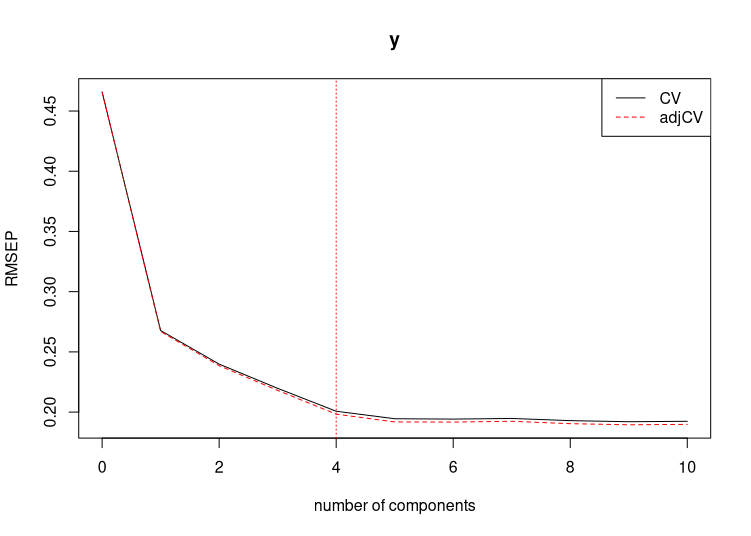
\includegraphics[width=0.5\linewidth]{rmse.png}}
        \subfloat[$R^2$\label{fig:r2}]{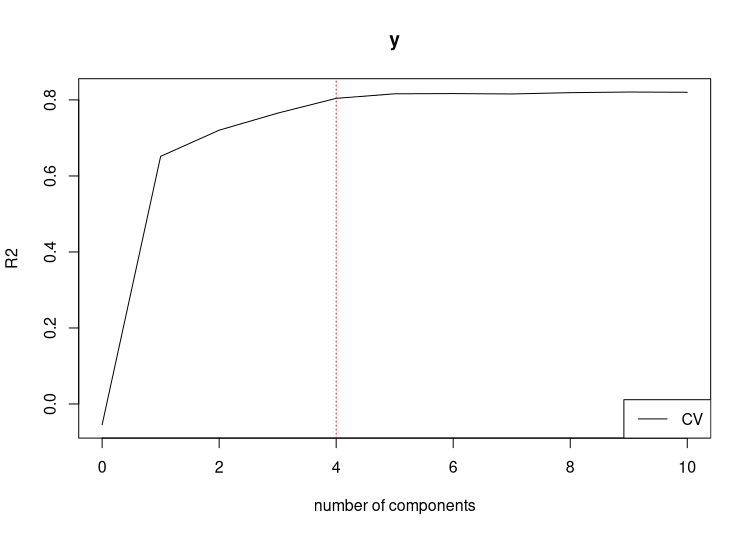
\includegraphics[width=0.5\linewidth]{r2.png}}
        \caption{In order to select the number of components to retain after Partial Least Squares Regression, the values of $RMSE$ and $R^2$ metrics are analysed. In both cases it's clearly visible that the improvement stops after the adding 4th component. Hence, for further experiments and prediction only 4 PLSR components will be used.}
        \label{fig:plsr}
    \end{figure}

    \begin{figure}
        \centering
        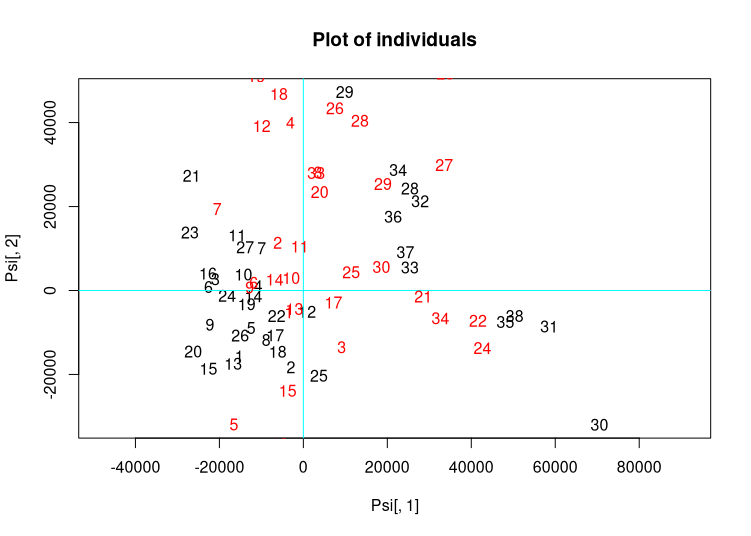
\includegraphics[width=\linewidth]{individuals.png}
        \caption{Test data, centered with respect to the mean of the training data, projected onto 4 selected PLSR components. Test data is shown in red color, whereas train data in black.}
        \label{fig:individuals}
    \end{figure}

\end{document}
